\subsection{Share of Detected Cases}
\label{subsec:results_share_known_cases}


This section shows the share of detected cases for different age groups. See
Section~\ref{sub:testing} for an explanation of how we model the detection of cases
and Section~\ref{subsec:data_share_known_cases} for the calibration of the relevant
parameters.

The share of detected cases fall drastically from October to December when the
incidence of CoViD-19 skyrocketed, PCR tests were still scarce and official contact
tracing became impossible due to the sheer amount of cases.

As rapid tests become available and more and more individuals receive positive rapid
tests and seek PCR tests, the share of detected cases starts to increase. While first
rapid tests are available since the beginning of 2021 the effect only becomes substantial
after March when access to rapid tests was greatly expanded.

Overall, the share of detected cases is much higher in older age groups. This is because
the likelihood to develop symptoms increases with age and symptomatic cases are
more likely to be detected.


A notable exception is that school age children (5-14, green line) overtake the next age
group in May 2021. This comes from a particularly strong increase in their share of
detected cases after Easter, when weekly rapid tests become mandatory in schools.

\begin{figure}[ht]
  \centering
  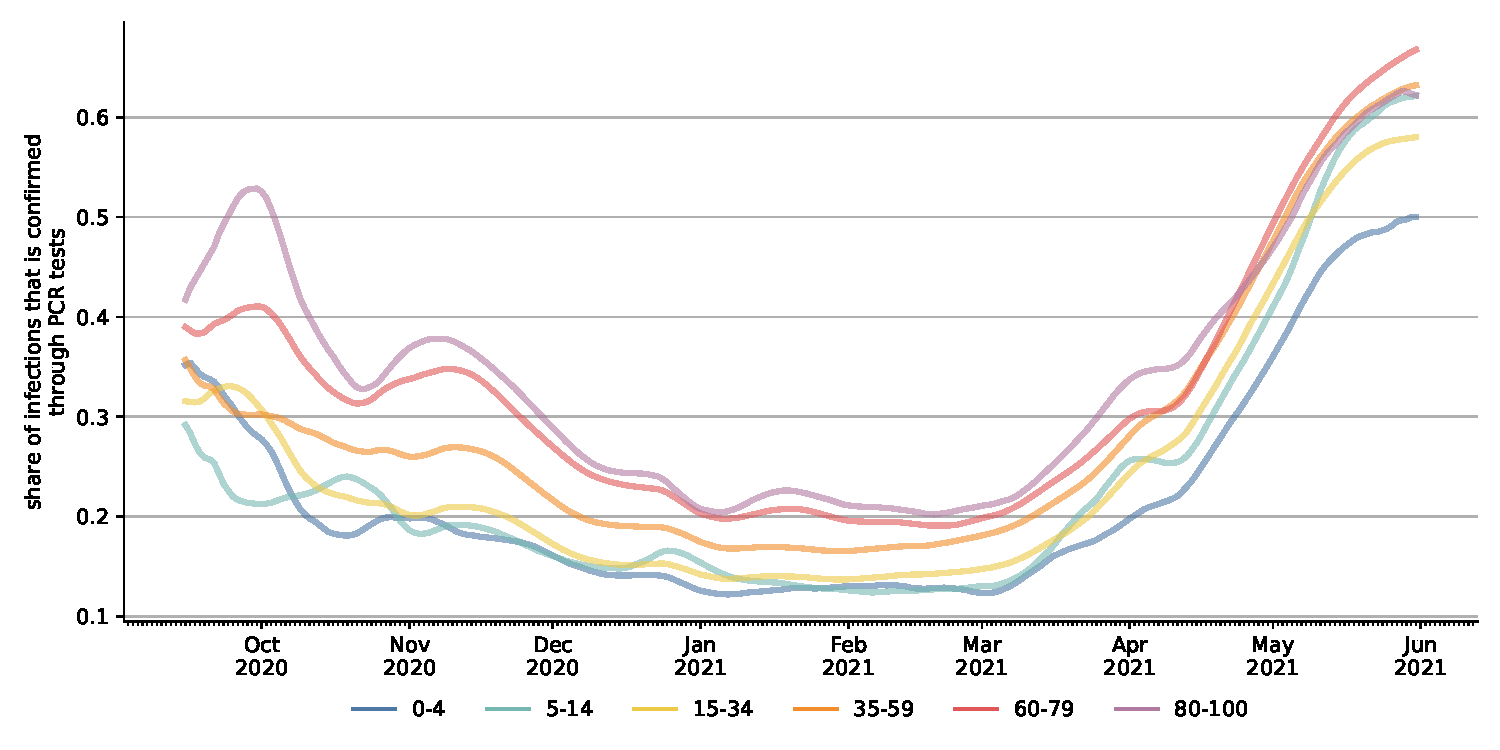
\includegraphics[width=0.5\textwidth]{figures/results/figures/share_known_cases/full_combined_baseline_by_age_group_rki}
  \caption{Share of Detected Cases by Age Group}
  \label{fig:share_known_cases_by_age_group}
  \floatfoot{\noindent \textit{Note:} The figure shows the share of cases that is
  reported as an official case for each age group in our simulated population. For
  legibility reasons, all lines are rolling 7-day averages of the average of 30
  simulation runs.}
\end{figure}


\FloatBarrier
